\documentclass{article}

\usepackage{graphicx} % Required for the inclusion of images
\usepackage{natbib} % Required to change bibliography style to APA

\setlength\parindent{0pt} % Removes all indentation from paragraphs

 \usepackage{url}

%----------------------------------------------------------------------------------------
%	Report on Argopy Project
%----------------------------------------------------------------------------------------

\title{Report on Argopy Project. \\ CMSC 6950} % Title

\author{Immanuel \textsc{Okpara}} % Author name

\date{\today} % Date for the report

\begin{document}

\maketitle % Insert the title, author and date

% If you wish to include an abstract, uncomment the lines below
% \begin{abstract}
% Abstract text
% \end{abstract}

%----------------------------------------------------------------------------------------
%	SECTION 1
%----------------------------------------------------------------------------------------

\section{Introduction}

Argo is a real-time global ocean observing system.

The Ocean makes up more than 70 percent of the earth's surface, and Argopy provides a global system for monitoring ocean behaviours.
Scientists study the behaviour of the Ocean for many reasons, including but not limited to;
\begin{enumerate}
    \item Ocean behaviour helps scientists understand global weather conditions.
    \item The Ocean supports different forms of life that need preserving; drastic changes in parameters like Temperature or Pressure will impact these life forms. 
    \item Global Warming
    \end{enumerate}
Argo consists of about 4000 autonomous floats, measuring parameters like Temperature, Pressure and Salinity. This historical data is available to the public through Agropy.
Argopy is an Ocean data analysis python package.\\

%----------------------------------------------------------------------------------------
%	SECTION 2
%----------------------------------------------------------------------------------------

\section{Installation}
Argopy is a python package and is compatible with python versions 3.6, 3.7 and 3.8. 
For this project, the following packages are required;

\begin{enumerate}
\item Argopy
\item Pandas 
\item Matplotlib
\item Numpy 
\end{enumerate}

%----------------------------------------------------------------------------------------
%	SECTION 3
%----------------------------------------------------------------------------------------

\section{Sample Data}

Each Argo float is autonomous and drifts the ocean freely. The float cannot control its position but can control its buoyancy. Each float moves up to the ocean's surface and then sinks to about 2000meters every ten days.
The figure below is data from 75W to 45W, 20N to 30N, 0db to 10db, January to June 2018 and July to December 2018. The Temperature data is plotted against time in the figures below.
\begin{figure}[h]
\begin{center}
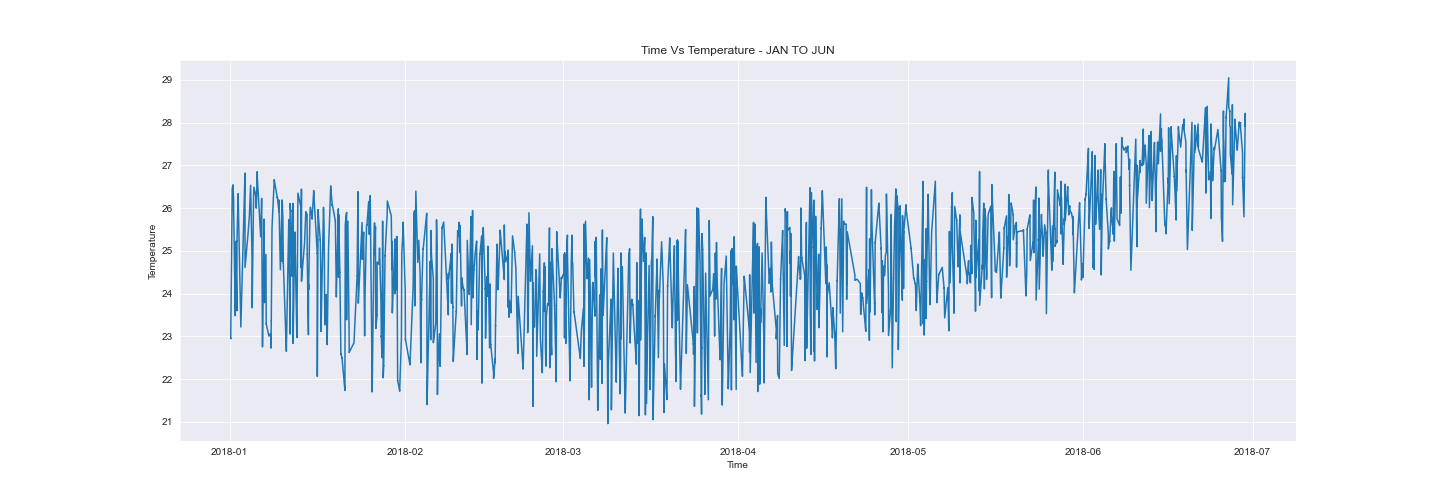
\includegraphics[width=1\textwidth]{JAN_JUN.png} % Include the image placeholder.png
\caption{JANUARY TO JUNE 2018.}
\end{center}
\end{figure}

\begin{figure}[h]
\begin{center}
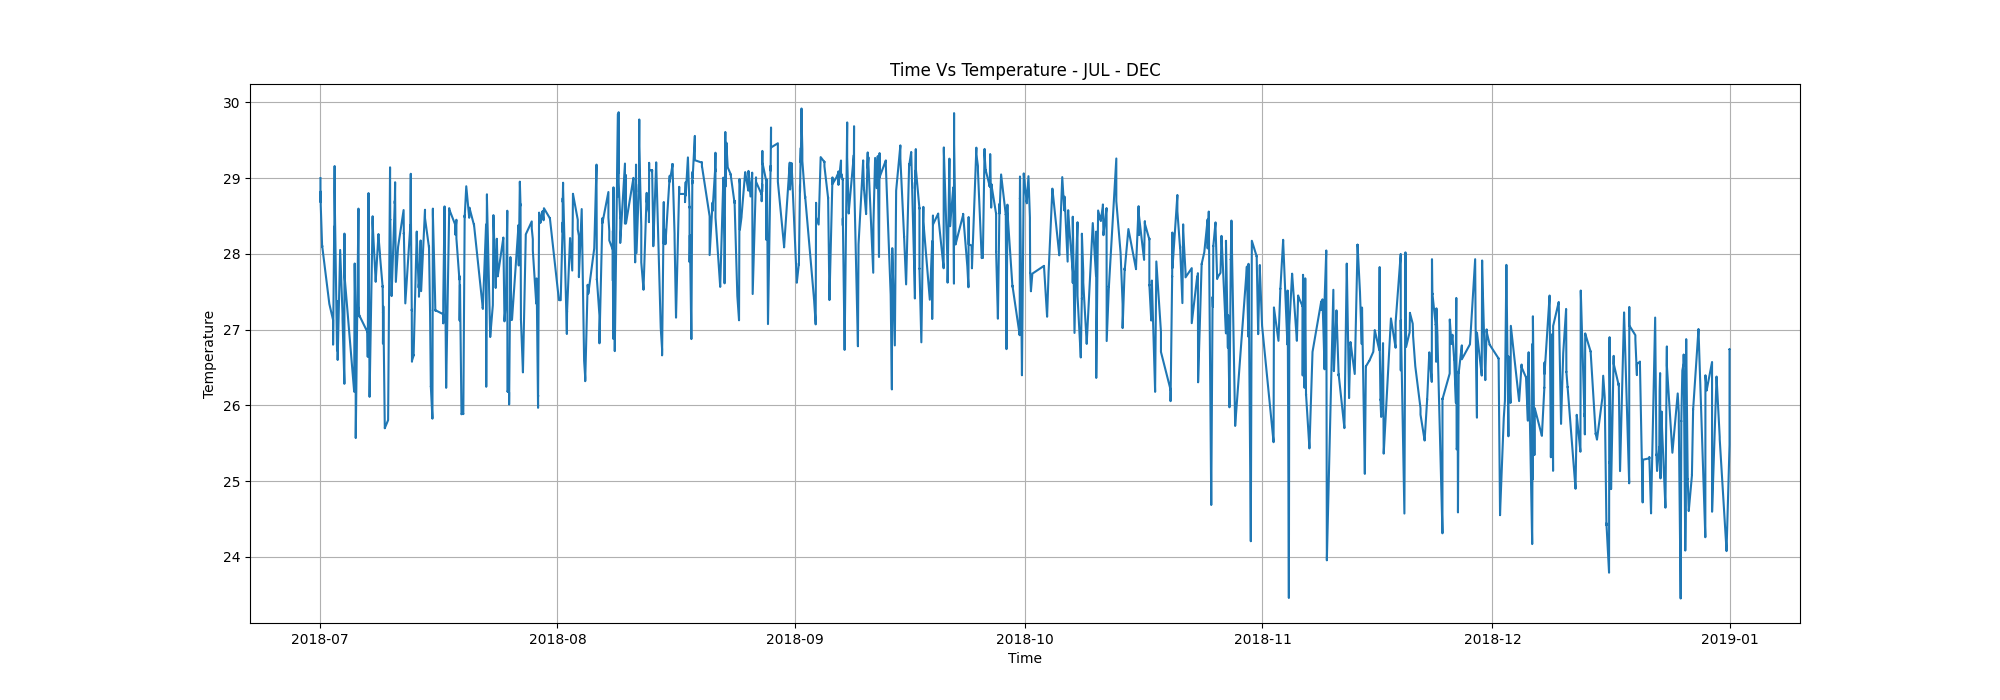
\includegraphics[width=1\textwidth]{JUL_DEC.png} % Include the image placeholder.png
\caption{JULY TO DECEMBER 2018}
\end{center}
\end{figure}

%----------------------------------------------------------------------------------------
%	SECTION 4
%----------------------------------------------------------------------------------------

\section{Results and Conclusion}
The zigzag pattern of the figures above represents the movement of the float every ten days. Temperatures start to  drop in August as winter season approaches.

There is a rise in Temperature from March, this represents the end of the winter and the beginning of the spring/summer season

%----------------------------------------------------------------------------------------
%	BIBLIOGRAPHY
%----------------------------------------------------------------------------------------

\section{BIBLIOGRAPHY}
\bibliographystyle{apalike}

\bibliography{sample}
\begin{enumerate}
\item Argo data python library - \url{ https://argopy.readthedocs.io/en/latest/index.html}
\end{enumerate}

%----------------------------------------------------------------------------------------


\end{document}